\documentclass[a4paper,10pt]{article}

\usepackage[T1]{fontenc}
\usepackage[utf8]{inputenc}
\usepackage[italian, english]{babel}
\usepackage{geometry}
\usepackage[hidelinks]{hyperref}
\usepackage{amsfonts}
\usepackage{amsmath}
\usepackage{amssymb}
\usepackage{tikz}
\usepackage{pgfplots}
\usepackage{fontawesome5}
\usepackage{graphicx}


\geometry{a4paper, top=2cm, bottom=2cm, left=2cm, right=2cm}
\pgfplotsset{compat=1.18}
\newcommand{\lambdabar}{\lambda\mkern-9mu\raisebox{0.4ex}{–}}
\newcommand{\B}{\boldsymbol}
\setlength\parindent{0pt}
\setlength{\parskip}{0.2em}
\graphicspath{{./Immagini/}}





\begin{document}

\title{\textbf{Esercizi Fisica Gravitazionale Avanzata}}
\author{Stefano Carturan - 49369A}
\date{\textit{Febbraio 2026}}
\maketitle

\tableofcontents

\newpage

\section{Onde gravitazionali}

Iniziamo leggendo la Sezione 8.1.1 del libro di Maggiore.
Consideriamo ora due masse $m_1$ e $m_2$, collegate da una molla di costante elastica $k$ lungo l’asse $x$.
Le oscillazioni sono smorzate da un attrito con $F = -a , dx/dt$. All’equilibrio le due masse si trovano a una distanza $L$.
Il sistema è investito da un’onda gravitazionale che si propaga nella direzione $z$, con
$h_{+} = h \cos(\omega t)$ lungo $x$ e $h_{\times} = 0$.

\begin{enumerate}

    \item Trova l’equazione del moto per $x(t)$. Dovrebbe assomigliare a quella di un oscillatore armonico smorzato, con una frequenza angolare non smorzata $\omega_0$ dipendente da $k$, $m_1$ e $m_2$, e un termine di sorgente dato dalle onde gravitazionali.
    
    \item Risolvi questa equazione nella forma $x(t) = A \cos(\omega t + \phi)$, e trova la frequenza di risonanza;
    
    \item Mediando su un’oscillazione, calcola l’energia totale del sistema e l’energia irradiata;
    
    \item Cosa succede qualitativamente se $h_{\times} \neq 0$ ma $h_{+} = 0$?

    \item Prendi $L = 10 \ \mathrm{m}$, $h = 10^{-21}$, $\omega_0 = 2\pi,\mathrm{kHz}$, $m_1 = m_2 = m = 10^3 \ \mathrm{kg}$, e un fattore di qualità $Q \sim 10^6$, vedi il Maggiore.
    Pensi che sia possibile rivelare onde gravitazionali con un sistema di questo tipo?

\end{enumerate}





\subsection{Equazione del moto}

Il problema descritto è un oscillatore armonico, posizionato lungo l'asse $x$, smorzato da una forza di attrito dovuta alla rigidità della molla e forzato dal passaggio di un'onda gravitazionale in direzione $-\hat z$. Rappresentiamo quindi la situazione descritta:

\begin{center}
\begin{tikzpicture}[scale=1.2]

\draw[->] (0,0,0) -- (6.5,0,0) node[right] {$x$};
\draw[->] (0,0,0) -- (0,2,0) node[above] {$y$};
\draw[->] (0,0,0) -- (0,0,5) node[above left] {$z$};

% masse
\draw[thick] (1.5,0,0) circle (0.2);
\node at (1.5,0.8,0) {$m_1$};
\draw[thick] (4,0,0) circle (0.5);
\node at (4,1.1,0) {$m_2$};

% molla
\draw[thick,decorate,decoration={coil,aspect=0.5,segment length=4pt,amplitude=4pt}]
(1.7,0,0) -- (3.5,0,0);
\node at (2.5,0.6,0) {$k$};

% GW
\draw[thick, ->] (3,0,4) -- (3,0,2);
\draw (2.8,0,3) -- (3.2,0,3) node[below right] {$h_+$};
\draw (3,-0.2,3) -- (3,0.2,3);

\end{tikzpicture}
\end{center}

%Per ricavare l'equazione del moto delle due masse, assumiamo che l'onda gravitazionale incida per un periodo di tempo sufficientemente lungo affinché la componente transiente del moto, determinata dall'attrito $-a \, dx/dt$, diventi trascurabile.
%Perciò faremo riferimento alla sezione 8.1.1 e 8.1.2 del Maggiore.
%Un'ulteriore assunzione va fatta per quanto riguarda le dimensioni del sistema rispetto alla lunghezza d'onda incidente: assumeremo $L \ll \lambdabar$, condizione che sperimentalmente è ragionevole ed è inoltre giustificata dai dati numerici forniti nell'ultimo punto del problema.

Per ricavare l'equazione del moto delle due masse, assumiamo che le dimensioni del sistema siano trascurabili rispetto alla scala di variazione del campo gravitazionale: assumiamo perciò $L \ll \lambdabar$.
Tale approssimazione è sperimentalmente ragionevole ed è inoltre giustificata dai dati numerici forniti nell'ultimo punto del problema.
In aggiunta, facendo riferimento alla sezione 1.3.3 del Maggiore, ci poniamo nel proper detector frame: così facendo possiamo utilizzare il fatto che l'equazione della deviazione geodetica si riduce a quella di una forza newtoniana (equazione 1.96).
Perciò abbiamo che la forzante dovuta all'onda gravitazionale agente sulla $k$-esima massa assume la forma:

\begin{equation} \label{eq:F}
    F_i^{(k)} = \frac{m^{(k)}}{2} \ddot{h}_{ij}^{TT} x^{(k) \, j} \ .
\end{equation}

Il problema, nel caso in cui sia presente la sola polarizzazione $h_+$ lungo l'asse $x$, risulta essere unidimensionale (lungo $\hat x$) e perciò consideriamo solamente tale componente nella precedente equazione:

\begin{equation} \label{eq:Fx}
    F_x^{(k)} = \frac{m^{(k)}}{2} \ddot{h}_+^{TT} x^{(k)} \ .
\end{equation}

Nelle equazioni \eqref{eq:F} e \eqref{eq:Fx}, la coordinata $x^{(k) \, 1} \equiv x^{(k)}$ è la posizione lungo l'asse $x$ della $k$-esima massa e, facendo riferimento al disegno, abbiamo assunto che l'origine del sistema di riferimento sia a sinistra della massa $m_1$, sufficientemente vicina a quest'ultima da poter comunque considerare la deviazione geodetica piccola rispetto alla lunghezza dell'onda gravitazionale: $x^{(k)} \simeq L \ll \lambdabar$.

Per studiare la dinamica del sistema, definiamo le coordinate baricentrali e relative come:

\begin{equation} \label{eq:coor}
\begin{aligned}
    \begin{cases}
        R = \dfrac{1}{M}(m_1 x_1 + m_2 x_2) \\[2mm]
        x = x_2 - x_1
    \end{cases}
    \qquad \qquad
    \begin{cases}
        M = m_1 + m_2 \\[2mm]
        \mu = \dfrac{m_1 m_2}{m_1 + m_2} \ .
    \end{cases}
\end{aligned}
\end{equation}

Scriviamo ora le equazioni del moto per entrambe le masse come quelle di due oscillatori smorzati e forzati:

\begin{equation} \label{eq:osillatori}
    \begin{cases}
        m_1 \ddot x_1 = -k(x_1 - x_2 - L) - a(\dot x_1 - \dot x_2) + \dfrac{m_1}{2} \ddot{h}_+^{TT} x_1 \\[2mm]
        m_2 \ddot x_2 = k(x_1 - x_2 - L) + a(\dot x_1 - \dot x_2) + \dfrac{m_2}{2} \ddot{h}_+^{TT} x_2 \ .
    \end{cases}
\end{equation}

Prendendone la somma e la differenza otteniamo:

\begin{equation} \label{eq:sommadiff}
    \begin{cases}
        m_1 \ddot x_1 + m_2 \ddot x_2 = \dfrac{1}{2} \ddot{h}_+^{TT} (m_1 x_1 + m_2 x_2) \\[2mm]
        m_2 \ddot x_2 - m_1 \ddot x_1 = 2k(x_1 - x_2 - L) + 2a(\dot x_1 - \dot x_2) + \dfrac{1}{2} \ddot{h}_+^{TT} (m_2 x_2 - m_1 x_1) \ .
    \end{cases}
\end{equation}

Considerando la seconda equazione, notiamo che\footnote{moltiplicando e dividendo per $M$, poi sommando e sottraendo $m_1 m_2 x_1 + m_1 m_2 x_2$.} $m_2 x_2 - m_1 x_1 = (m_2 - m_1)R + 2\mu x$.
Riscriviamo le due equazioni in termini delle coordinate \eqref{eq:coor} ed utilizziamo la prima equazione per eliminare dalla seconda i gradi di libertà del centro di massa.
Otteniamo così un sistema di due equazioni differenziali disaccoppiate, una per la posizione del centro di massa $R$ ed una per la posizione relativa $x$:

\begin{equation} \label{eq:sommadiffrel}
    \begin{cases}
        \ddot R = \dfrac{1}{2} \ddot{h}_+^{TT} R \\[2mm]
        \mu \ddot x = -k (x-L) - a \dot x + \dfrac{\mu}{2} \ddot{h}_+^{TT} x \ .
    \end{cases}
\end{equation}

Osserviamo che la dinamica di interesse è descritta dall'equazione per la coordinata relativa, perciò ci concentreremo sulla seconda equazione del sistema \eqref{eq:sommadiffrel}, definendo la frequenza propria dell'oscillatore $\omega_0^2 \equiv \frac{k}{\mu}$ e la costante di smorzamento della molla $\gamma \equiv \frac{a}{2\mu}$.
Notando infine che $\ddot{h}_+^{TT} = -\omega^2{h}_+^{TT}$, otteniamo l'equazione del moto richiesta:

\begin{equation} \label{eq:eqmoto}
    \ddot x = -\omega_0^2 (x-L) - 2\gamma \dot x - \frac{1}{2} \omega^2 h_+^{TT} x \ ,
\end{equation}

che, come anticipato, rappresenta un oscillatore armonico di frequenza $\omega_0$ forzato da un termine $\propto h_+^{TT}$, dovuto al passaggio dell'onda gravitazionale, e smorzato da un termine $\propto a$.





\subsection{Legge oraria}

Per risolvere l'equazione del moto \eqref{eq:eqmoto} del sistema, conviene riscriverla definendo la posizione relativa come: $x = L + r$, dove il termine $r$ è una perturbazione alla posizione di equilibrio di ordine $h$.
Con questo cambio di variabile otteniamo:

\begin{equation} \label{eq:oscill}
    \ddot r + 2 \gamma \dot r + \omega_0^2 r = - \frac{h}{2} \omega^2 L \cos(\omega t) \ ,
\end{equation}

dove nel termine forzante abbiamo trascurato il contributo $h r = \mathcal O(h^2)$. L'equazione, come già detto, è quella di un oscillatore armonico smorzato e forzato, la cui soluzione è data dalla combinazione della soluzione dell'equazione omogenea associata e di una soluzione particolare.
Cominciamo col risolvere l'equazione omogenea associata:

\begin{equation} \label{eq:omog}
    \ddot r + 2 \gamma \dot r + \omega_0^2 r = 0
\end{equation}

con una funzione del tipo: 

\begin{equation} \label{eq:ansatzomog}
    \tilde r(t) = e^{\lambda t} \ ,
\end{equation}

dove $\lambda \in \mathbb C$.
Il polinomio caratteristico $\lambda^2 + 2\gamma \lambda + \omega_0^2$ ha due radici: $\lambda_{+,-} = -\gamma \pm \sqrt{\gamma^2 - \omega_0^2}$ e, in base al valore del dell'argomento della radice, possiamo distinguere tre casi.
Se $\gamma^2 > \omega_0^2$ siamo in regime sovrasmorzato, se $\gamma^2 = \omega_0^2$ siamo nel caso criticamente smorzato, mentre se $\gamma^2 < \omega_0^2$ l'oscillatore è sottosmorzato; vedremo che proprio quest'ultimo è il caso di nostro interesse.
In tutti e tre i casi, ad ogni modo, la parte reale dell'esponente $\lambda$ nella $\eqref{eq:ansatzomog}$ sarà negativa, e perciò la soluzione dell'equazione omogenea $\tilde r(t)$ è un transiente che a regime diventerà trascurabile.
In particolare, scrivendo la soluzione dell'omogenea per il caso sottosmorzato:

\begin{equation} \label{eq:sottosmorz}
    \tilde r(t) = \tilde A e^{-\gamma t} \cos(\tilde \omega t + \tilde \phi) \ ,
\end{equation}

dove $\tilde \omega = \sqrt{\omega_0^2 - \gamma^2}$, notiamo che essa decresce esponenzialmente con un tempo scala $\tau = \gamma^{-1}$.

Passiamo ora alla soluzione particolare dell'equazione \eqref{eq:oscill}, facendo l'ipotesi che essa abbia la seguente forma:

\begin{equation} \label{eq:ansatz}
    r(t) = A \cos(\omega t + \phi) \ .
\end{equation}

Possiamo vedere $r(t)$ come la parte reale di una soluzione complessa $z(t) = r(t) + iy(t) = A e^{i(\omega t + \phi)}$. In tal modo, l'equazione \eqref{eq:oscill} diventa:

\begin{equation} \label{eq:complessa}
    \text{Re} \left\{ \ddot z + 2 \gamma \dot z + \omega_0^2 z \right\} = \text{Re} \left\{ - \frac{h}{2} \omega^2 L e^{i \omega t} \right\} \ .
\end{equation}

Svolgendo le derivate, possiamo raccogliere e semplificare un termine $e^{i \omega t}$, rimanendo con la seguente equazione:

\begin{equation}
    A e^{i \phi} (- \omega^2 + 2i \gamma \omega + \omega_0^2) = - \frac{h}{2} \omega^2 L \ ,
\end{equation}

che, scomposta nuovamente in parte reale e immaginaria, dà luogo al seguente sistema:

\begin{equation} \label{eq:sistemaphi}
\begin{cases}
    \cos(\phi) = \dfrac{2A}{h \omega^2 L} (\omega_0^2 - \omega^2) \\[2mm]
    \sin(\phi) = \dfrac{4A \gamma}{h \omega L} \ .
\end{cases}
\end{equation}

Possiamo quindi trovare la fase iniziale $\phi$ e l'ampiezza $A$ della soluzione \eqref{eq:ansatz}:

\begin{equation}
\begin{cases}
    \phi = \arctan \left( \dfrac{2 \gamma \omega}{\omega^2 - \omega_0^2} \right) \\[3mm]
    A = \dfrac{hL}{2} \dfrac{\omega^2}{\sqrt{(\omega_0^2 - \omega^2)^2 + 4 \gamma^2 \omega^2}} \ .
\end{cases}
\end{equation}

Notiamo che esse non dipendono dalle condizioni iniziali in cui è stato posto il sistema in quanto, come abbiamo visto, il contributo alla soluzione dato dall'equazione omogenea associata è un transiente e perciò la soluzione a regime, ossia per $t \gg \tau = \gamma^{-1}$, coincide con la soluzione particolare \eqref{eq:ansatz}:

\begin{equation}
    r(t) = \dfrac{hL}{2} \dfrac{\omega^2}{\sqrt{(\omega_0^2 - \omega^2)^2 + 4 \gamma^2 \omega^2}} \cos \left( \omega t + \arctan \left( \dfrac{2 \gamma \omega}{\omega^2 - \omega_0^2} \right) \right) \ .
\end{equation}

Inoltre, notiamo che l'ampiezza di oscillazione $A(\omega)$ presenta un massimo\footnote{il massimo si calcola ponendo a zero la derivata di $A$ rispetto a $\omega$.} alla frequenza:

\begin{equation} \label{eq:wrisonanza}
    \omega_R = \omega_0 \left( 1 - \frac{2 \gamma^2}{\omega_0^2} \right)^{-\frac{1}{2}} \ ,
\end{equation}

che chiamiamo frequenza di risonanza.
Per completezza, ricordiamo che la soluzione completa dell'equazione del moto \eqref{eq:eqmoto} è:

\begin{equation} \label{eq:leggeoraria}
    x(t) = r(t) + L \ .
\end{equation}





\subsection{Energia totale e irradiata}

Date l'equazione del moto \eqref{eq:eqmoto} e la su soluzione \eqref{eq:leggeoraria}, possiamo calcolare l'energia totale del sistema come somma di un contributo cinetico e di uno potenziale:

\begin{equation} \label{eq:energia}
\begin{aligned}
    E(t)    &= T(t) + U(t) = \frac{1}{2} \mu \dot x^2(t) + \frac{1}{2} k [x(t) - L]^2 = \frac{1}{2} [\mu \dot r^2(t) + k r^2(t)] = \\
            &= \frac{A^2}{2} [\mu \omega^2 \sin^2(\omega t + \phi) + k \cos^2(\omega t + \phi)] \ .
\end{aligned}
\end{equation}

Così facendo stiamo calcolando l'energia dell'oscillatore a regime, ovvero trascurando i contributi transienti per $t \gg \tau$: in altre parole stiamo assumendo che tutta l'energia fornita al sistema dall'onda gravitazionale incidente venga utilizzata per compensare la dissipazione dovuta alla non idealità della molla, trascurando altri termini dissipativi, come ad esempio l'emissione di onde gravitazionali da parte del sistema stesso.
L'energia in funzione del tempo oscilla con periodo $T=\frac{2\pi}{\omega}$, perciò ne possiamo calcolare la media su un periodo, che corrisponde ad un'oscillazione completa delle due masse:

\begin{equation} \label{eq:energiaperiodo}
    \langle E \rangle_T = \frac{1}{T} \int_0^T E(t) dt = \frac{A^2}{2} \frac{\omega}{2\pi} \int_0^{2\pi/\omega} [\mu \omega^2 \sin^2(\omega t + \phi) + k \cos^2(\omega t + \phi)] dt \ .
\end{equation}

Sapendo che $\frac{1}{T}\int_0^T\sin^2(x)dx = \frac{1}{T}\int_0^T\cos^2(x)dx = \frac{1}{2}$, l'energia media diventa:

\begin{equation} \label{eq:energiamediaperiodo}
    \langle E \rangle_T = \frac{A^2 \mu}{4} (\omega^2 + \omega_0^2) = \frac{\mu h^2 L^2 \omega^4}{16} \frac{\omega^2 + \omega_0^2}{(\omega_0^2 - \omega^2)^2 + 4 \gamma^2 \omega^2} \ .
\end{equation}

Come abbiamo detto, in questo calcolo finora abbiamo trascurato l'emissione di energia sotto forma di onde gravitazionali prodotte dall'oscillazione delle due masse, perciò ora andremo a calcolare proprio questo effetto.
Per calcolare l'energia totale irradiata partiremo dalla potenza, seguendo l'approccio del problema 3.1 del Maggiore.
La potenza irraggiata per unità di angolo solido in approssimazione di quadrupolo per un sistema di due masse connesse da una molla lungo l'asse $x$ è data dall'equazione 3.314:

\begin{equation} \label{eq:potangsolido}
    \left( \frac{dP}{d\Omega} \right)_{\text{q}} = \frac{r^2 c^3}{16 \pi G} \langle \dot h_+^2 \rangle \ ,
\end{equation}

dove $r$ è la distanza dalla sorgente. L'ampiezza $h_+$ è calcolata a partire dall'equazione 3.72 del Maggiore, considerando che, nel nostro caso, è conveniente definire l'angolo polare $\theta$ del sistema di coordinate sferiche a partire dall'asse $x$ ($\theta=0$), mentre l'angolo azimutale $\varphi$ descrive le rotazioni nel piano $z-y$, sotto le quali la potenza irradiata è invariante.
In tale sistema di riferimento, il termine $M_{33}$ nell'equazione 3.72 diventa $M_{11}$, e questo è l'unico contributo che non si annulla.
Infatti:

\begin{equation} \label{eq:Mij}
    M^{ij}(t) = \int d^3\boldsymbol x \rho(t, \boldsymbol x) x^i x^j = \int d^3\boldsymbol x \mu \delta_D \big( x - x(t) \big) \delta_D(y) \delta_D(z) x^i x^j = \mu x^2(t) \delta^{i1} \delta^{j1}
\end{equation}

dove $x(t)$ è data dalla \eqref{eq:leggeoraria}. Dunque, dall'equazione 3.322 del Maggiore, si ha:

\begin{equation} \label{eq:hplus}
    h_+(t, \theta, \varphi) = \frac{2G \mu \omega^2}{r c^4} \sin^2(\theta) [A^2 \cos(2 \omega t_{r}) + LA \cos(\omega t_r)] \ ,
\end{equation}

dove $t_r$ è il tempo ritardato a cui viene rilevato il segnale. Derivando nel tempo ed elevando al quadrato si ottiene:

\begin{equation} \label{eq:hplusdot2}
    \dot h_+^2(t, \theta, \varphi) = \frac{4 G^2 \mu^2 A^2 \omega^6}{r^2 c^8} \sin^4 (\theta) [4A^2 \sin^2(2\omega t_r) + 4AL \sin(\omega t_r) \sin(2 \omega t_r) + L^2 \sin^2(\omega t_r)] \ .
\end{equation}

Per calcolare il valore medio $\langle \dot h_+^2 \rangle$, bisogna integrare su un periodo della funzione $\dot h_+^2$, che vale $T=\frac{2\pi}{\omega}$, nel farlo, il doppio prodotto si annulla, perciò troviamo:

\begin{equation} \label{eq:hdotmedio}
\begin{aligned}
    \langle \dot h_+^2 \rangle  &= \frac{1}{T} \int_0^T \dot h_+^2 dt = \\
                                &= \frac{4 G^2 \mu^2 A^2 \omega^6}{r^2 c^8} \sin^4 (\theta) \left[ 4A^2 \frac{1}{T} \int_0^T \sin^2(2\omega t) dt + L^2 \frac{1}{T} \int_0^T \sin^2(\omega t) dt \right] \ ,
\end{aligned}
\end{equation}

dove abbiamo sostituito il tempo ritardato $t_r = t + r/c$ con $t$ perché lo sfasamento di un valore costante non cambia il valore dell'integrale sul periodo.
Come visto in precedenza, $\frac{1}{T}\int_0^T\sin^2(x)dx = \frac{1}{2}$, tuttavia il primo seno che compare nell'equazione \eqref{eq:hdotmedio} ha un periodo di $\frac{\pi}{\omega}$, perciò:

\begin{equation} \label{eq:integraleperiodo}
    \frac{1}{T}\int_0^T\sin^2(2 \omega t)dt = \frac{\omega}{2 \pi} \left[ \int_0^{\pi/\omega} \sin^2(2\omega t) dt + \int_{\pi/\omega}^{2\pi/\omega} \sin^2(2\omega t) dt \right] = \frac{\omega}{2 \pi} \left[ \frac{\pi}{2 \omega} + \frac{\pi}{2 \omega} \right] = \frac{1}{2} \ .
\end{equation}

Dunque, la potenza irradiata per unità di angolo solido in approssimazione di quadrupolo è:

\begin{equation} \label{eq:potenzaperanglosolido}
    \left( \frac{dP}{d\Omega} \right)_{\text{q}} = \frac{G \mu^2 A^2 \omega^6}{8 \pi c^5} \sin^4(\theta) [4A^2 + L^2]
\end{equation}

Per trovare la potenza totale irradiata, integriamo sull'angolo solido:

\begin{equation} \label{eq:potenzatot}
    P_q = \int d\Omega \left( \frac{dP}{d\Omega} \right)_{\text{q}} = \frac{G \mu^2 A^2 \omega^6}{4 c^5} \frac{2\pi}{2\pi} \int_0^\pi \sin^5(\theta) d\theta \, [4A^2 + L^2] = \frac{4 G \mu^2 A^2 \omega^6}{15 c^5} [4A^2 + L^2] \ .
\end{equation}

Ed infine, integrando nuovamente sul periodo $T=\frac{2\pi}{\omega}$ otteniamo l'energia totale irradiata in un'oscillazione del sistema sotto forma di onde gravitazionali:

\begin{equation} \label{eq:energiairradiata}
    E_q = \int_0^{2\pi/\omega} P dt = \frac{8 \pi}{15} \frac{G \mu^2 A^2 \omega^5}{c^5} [4A^2 + L^2] = \frac{32 \pi}{15} \frac{G \mu^2}{A} \left( \frac{v}{c} \right)^5 \left[ 1 + \frac{L^2}{4A^2} \right] \ ,
\end{equation}

che scala come $(v/c)^5$, dove $v = A\omega$.




\subsection{Cambio di polarizzazione}

In questo esercizio abbiamo considerato l'effetto di un'onda gravitazionale su un sistema con scala $L \ll \lambdabar$.
Tale approssimazione ci ha permesso di trattare l'azione dell'onda come una forza newtoniana diretta lungo l'asse $x$ a causa della presenza del solo contributo $h_+$ alla polarizzazione.
Se ora supponiamo di avere $h_+ = 0$ e $h_\times \ne 0$, il pattern di linee di forza con cui possiamo schematizzare l'effetto dell'onda gravitazionale viene ruotato di $45^\circ$, come rappresentato nel seguente disegno. 


\begin{center}
\begin{tikzpicture}[scale=2]

\usetikzlibrary{decorations.markings}

\tikzset{
    freccia_avanti/.style={
        postaction={decorate},
        decoration={
            markings,
            mark=at position 0.5 with {\arrow{stealth}}
        }
    }
}

\tikzset{
    freccia_indietro/.style={
        postaction={decorate},
        decoration={
            markings,
            mark=at position 0.5 with {\arrow{stealth reversed}}
        }
    }
}

% Assi
\draw[->] (-2,0) -- (2,0) node[right] {$x$};
\draw[->] (0,-2) -- (0,2) node[above] {$y$};

% x^2 - y^2 = 1  --> y = ±sqrt(x^2 -1)
\draw[thick, blue, freccia_avanti, domain=1:2, samples=200]
plot (\x,{sqrt(\x*\x -1)}) -- (2,1.732);
\draw[thick, blue, freccia_indietro, domain=1:2, samples=200]
plot (\x,{-sqrt(\x*\x -1)}) -- (2,-1.732);

\draw[thick, blue, freccia_avanti, domain=-2:-1, samples=200]
plot (\x,{sqrt(\x*\x -1)}) -- (-1,0);
\draw[thick, blue, freccia_indietro, domain=-2:-1, samples=200]
plot (\x,{-sqrt(\x*\x -1)}) -- (-1,0);

% y^2 - x^2 = 1  --> x = ±sqrt(y^2 -1)
\draw[thick, blue, freccia_avanti, domain=1:2, samples=200]
plot ({sqrt(\x*\x -1)},\x) -- (1.5,1.802);
\draw[thick, blue, freccia_indietro, domain=1:2, samples=200]
plot ({-sqrt(\x*\x -1)},\x) -- (-1.5,1.802);

\draw[thick, blue, freccia_avanti, domain=-2:-1, samples=200]
plot ({sqrt(\x*\x -1)},\x) -- (0,-1);
\draw[thick, blue, freccia_indietro, domain=-2:-1, samples=200]
plot ({-sqrt(\x*\x -1)},\x) -- (0,-1);


% masse
\draw[thick] (-1,0,0) circle (0.05);
\node at (-1.3,0.2,0) {$m_1$};
\draw[thick] (1,0,0) circle (0.05);
\node at (1.3,0.2,0) {$m_2$};

% molla
\draw[thick,decorate,decoration={coil,aspect=0.5,segment length=4pt,amplitude=4pt}]
(-0.95,0,0) -- (0.95,0,0);
\node at (0.2,0.2,0) {$k$};

%forze
\draw[<-, thick, red] (-1,-0.4) -- (-1,0);
\draw[->, thick, red] (1,0) -- (1,0.4);
\node at (0.5,1.4) {$h_\times$};

\end{tikzpicture}
\end{center}

Da tale grafico possiamo intuire che, al primo ordine in $h$, le due masse sentano delle forze le quali, essendo tangenti alle linee di forza rappresentate, risultano essere parallele all'asse $y$.
Inoltre, quando la massa $m_1$ viene tirata in basso, la massa $m_2$ sente una forza verso l'alto e viceversa.
Perciò le due masse inizieranno ad oscillare in controfase sull'asse $y$, mantenendo in prima approssimazione invariata la loro distanza relativa orizzontale: $|x_2 - x_1| = L$.

Siccome le due masse sono diverse, avranno ampiezze di oscillazione differenti e questo, unito al fatto che il centro di massa del sistema non è esattamente a metà della distanza relativa tra le due molle, renderà instabile questa oscillazione lungo $y$.
Ci aspettiamo tuttavia che questa instabilità sia governata da effetti di ordine superiore ad $\mathcal O(h)$.




\subsection{Risultati osservativi}

Calcoliamo l'ampiezza delle oscillazioni del sistema alla frequenza di risonanza $\omega_R \simeq \omega_0 \simeq 2\pi \times 10^3$ Hz per capire se sia possibile rilevare o meno le oscillazioni del sistema:

\begin{equation} \label{eq:risonanza}
    A_R = \frac{h L}{4} \frac{\omega_0^2}{\gamma \sqrt{\omega_0^2 - \gamma^2}} = \frac{h L}{2} \frac{Q}{\sqrt{1 - \frac{1}{4Q^2}}} \simeq \frac{h L Q}{2} = 0.5 \times 10^{-14} \text{ m .}
\end{equation}

Un fattore di qualità di $10^6$ si può ottenere solo per temperature criogeniche, $T \simeq 10$ K (si veda la sezione 8.1.1 del Maggiore). 
A queste temperature il rumore termico ha un'energia di scala pari a $E_T \simeq k_B T \simeq 1.38 \times 10^{-22}$ J, che tuttavia è di molto inferiore all'energia cinetica del nostro sistema; infatti, dall'equazione \eqref{eq:energiamediaperiodo}, otteniamo un contributo alla risonanza pari a:

\begin{equation} \label{eq:epotrisonanza}
    T_R = \frac{A_R^2 \mu}{4} \omega_R^2 \simeq \frac{A_R^2 m}{8} \omega_0^2 \simeq 1.23 \times 10^{-19} \text{ J .}
\end{equation}

Perciò il rumore termico è ininfluente rispetto all'oscillazione delle due masse. 

Dopo un certo intervallo di tempo, il segnale dovuto all'onda gravitazionale cesserà, allora le oscillazioni verranno smorzate di un fattore $\gamma$. 
Dalla definizione del fattore di qualità $Q = \omega_0/2\gamma$, possiamo ricavare un ordine di grandezza per il tempo di smorzamento delle oscillazioni:

\begin{equation} \label{eq:tau}
    \tau = \frac{1}{\gamma} = \frac{2 Q}{\omega_0} \simeq 0.32 \times 10^3 \text{ s .}
\end{equation}

Questo tempo di rilassamento ci permetterebbe di misurare la differenza tra lo stato di quiete e di moto oscillatorio del sistema.

I moderni interferometri, come LIGO, sono sensibili a frequenze basse, in un range tra i le decine e le centinaia di Hz, poiché a frequenze superiori lo shot noise dei fotoni abbatte la sensibilità dello strumento.
I detector a massa risonante, come quello schematizzato in questo esercizio, invece, sono sensibili ad un piccolo intervallo di frequenze centrato sulla loro frequenza di risonanza, tipicamente di ordine del kHz, perciò in linea di principio potrebbero osservare onde gravitazionali a frequenze maggiori degli interferometri. 
Tuttavia, onde gravitazionali con ampiezze simili a quella data ($h\simeq 10^{-21}$) sono emesse tipicamente dal collasso di binarie compatte, che però ha frequenze che variano all'incirca tra $1$ e $100$ Hz.
Osservativamente si vede che, al crescere della frequenza tipica di un'onda gravitazionale, la sua ampiezza diminuisce: per esempio le pulsars emettono onde con $\omega_P \simeq 10^{-5} - 10^{-4}$ Hz e $h_P \simeq 10^{-14}$, i SMBH sono caratterizzati da $\omega_{SMBH} \simeq 10^{-4} - 1$ Hz e $h_{SMBH} \simeq 10^{-18}$ e, come detto, il collasso di binarie compatte presenta $\omega_{CB} \simeq 1 - 10^{2}$ Hz e $h_{CB} \simeq 10^{-21}$.
Quindi probabilmente se esistesse una sorgente $X$, caratterizzata da $\omega_X \simeq 10^{3}$ Hz e $h_X \simeq 10^{-21}$, le onde gravitazionali prodotte da tale sorgente sarebbero rilevabili con un detector a massa risonante.

In ultimo, verifichiamo che le assunzioni fatte per risolvere questo esercizio siano consistenti.

\begin{itemize}

    \item La prima e più importante assunzione che abbiamo fatto, è stata quella di considerare la taglia del sistema molto minore della scala di variazione del campo gravitazionale dovuta alla presenza dell'onda, ovvero che $L \ll \lambdabar$.
        Dai dati forniti, considerando che l'onda incidente abbia $\omega = \omega_R \simeq \omega_0$ abbiamo $L = 10$ m e $\lambdabar \simeq c/\omega_0 \simeq 0.48 \times 10^5$ m, per cui l'assunzione che abbiamo fatto è giustificata.

    \item Nella derivazione dell'equazione del moto, abbiamo assunto un segnale periodico, perciò abbiamo supposto che l'onda incida sul sistema per un tempo molto maggiore del tempo scala di dissipazione delle oscillazioni dovuto all'attrito.
        In altre parole, l'equazione del moto \eqref{eq:eqmoto} è valida solo se il segnale dura un tempo $\Delta t \gg \tau$, con $\tau$ dato dall'equazione \eqref{eq:tau}, che vale $\tau \simeq 0.32 \times 10^3$ s. Inoltre dall'equazione \eqref{eq:tau}, vediamo che $\omega_0 = 2Q \gamma$, perciò siamo nel caso di un moto oscillatorio sottosmorzato. 
    
    \item Un'altra assunzione è stata quella di trascurare l'energia emessa dal sistema in oscillazione sotto forma di onde gravitazionali nel calcolo dell'energia totale.
        Confrontiamo quindi i valori numerici delle energie espresse dalle equazioni \eqref{eq:energiamediaperiodo} e \eqref{eq:energiairradiata}: la prima restituisce l'energia totale del sistema (cinetica più potenziale) mediata su un'oscillazione, che alla risonanza vale $\langle E \rangle_T \simeq 2T_R \simeq 2.46 \times 10^{-19}$ J, mentre la seconda rappresenta l'energia persa dal sistema a causa della sua emissione di onde gravitazionali in un periodo, che alla risonanza vale $E_q \simeq 2.81 \times 10^{-58}$ J.
        Anche in questo caso possiamo dire di avere effettuato un'approssimazione più che ragionevole. 

\end{itemize}




\newpage

\section{Cosmologia}

Tutta la luce nell’Universo viene deviata, in particolare quei fotoni che viaggiano più a lungo come quelli della CMB.
In questo esercizio vogliamo comprendere le basi del lensing della CMB.

\begin{enumerate}

    \item Verifica tutte le equazioni nella Sezione 13.3 del Dodelson \& Schmidt, sul lensing della CMB.
    Potresti aver bisogno di espressioni aggiuntive da altre parti dello stesso capitolo.

    \item Calcola lo spettro di potenza lensato della temperatura della CMB utilizzando l’Eq. 13.21.
    In linea di principio potresti calcolare lo spettro di potenza del lensing a partire dallo spettro di potenza allegato a $z = 0$ e dal seguente background cosmologico: $\Omega_m = 0.3$, $\Omega_\Lambda = 1 - \Omega_m - \Omega_r$, dove la radiazione corrisponde a un corpo nero con temperatura $T_0 = 2.7$ K.
    Il valore della costante di Hubble è $H_0 = 68$ km/s/Mpc.
    Troverai anche lo spettro di potenza del lensing della CMB nei file allegati.
    Quest’ultimo potrebbe differire dal tuo calcolo a bassi $\ell$ a causa di alcune approssimazioni fatte nella Sezione 13.3, ma i due dovrebbero essere globalmente consistenti.

    \item Ripeti il primo punto per la polarizzazione della CMB. Questa volta ciò che viene traslato è il tensore di polarizzazione $I_{ij}$.
    Assumendo che non ci siano modi B iniziali, calcola lo spettro di potenza risultante per i modi E e B. Rappresenta graficamente i risultati.

\end{enumerate}


\subsection{Equazioni della Sezione 13.3 del Dodelson}

\subsubsection*{Equazione 13.18}

\begin{equation} \label{eq:13.18}
    T_{\mathrm{obs}}(\B\theta) = T(\B\theta + \Delta \B\theta[\B\theta])
        \simeq T(\B\theta) + \Delta \theta^i \frac{\partial}{\partial \theta^i} T(\B\theta) + \frac{1}{2} \Delta \theta^i \Delta \theta^j \frac{\partial^2}{\partial \theta^i \partial \theta^j} T(\B\theta) \ .
\end{equation}

È lo sviluppo di Taylor al secondo ordine della distribuzione di temperatura $T$ al variare dell'angolo $\B\theta$ bidimensionale, calcolato in approssimazione di cielo piatto. 
Con $T(\B \theta)$ si intende la distribuzione di temperatura al momento di emissione della CMB. \hfill $\blacksquare$





\subsubsection*{Equazione 13.19}

\begin{equation} \label{eq:13.19}
    \Delta \B{\theta}(\B l) = i \, \B l \, \phi_L(\B l) \ .
\end{equation}

È una relazione in spazio di Fourier coniugata alla 13.15 in spazio reale:

\begin{equation} \label{eq:13.15}
    \Delta \theta^i (\B\theta) = \frac{\partial}{\partial \theta^i} \phi_L(\B \theta) \ .
\end{equation}

Esprimiamo $\phi_L(\B \theta)$ e $\Delta \theta^i (\B\theta)$ come antitrasformate di Fourier:

\begin{equation} \label{eq:phideltafourier}
\begin{cases}
    \phi_L(\B \theta) = \displaystyle \int \frac{d^2 \B l}{(2\pi)^2} \phi_L(\B l) e^{i \B l \cdot \B \theta} \\[3mm]
    \Delta \theta^i (\B\theta) = \displaystyle \int \frac{d^2 \B l}{(2\pi)^2} \Delta \theta^i (\B l) e^{i \B l \cdot \B \theta} \ .
\end{cases}
\end{equation}

Prendiamo l'equazione \eqref{eq:13.15} e sostituiamo $\phi_L$ con la sua espressione in spazio di Fourier:

\begin{equation}
    \Delta \theta^i (\B\theta) = 
    \frac{\partial}{\partial \theta^i} \displaystyle \int \frac{d^2 \B l}{(2\pi)^2} \phi_L (\B l) e^{i \B l \cdot \B \theta} = 
    \displaystyle \int \frac{d^2 \B l}{(2\pi)^2} \phi_L (\B l) i  l^i e^{i \B l \cdot \B \theta} \ .
\end{equation}

Confrontando quest'ultima con l'espressione di $\Delta \theta^i (\B\theta)$ data dalla \eqref{eq:phideltafourier}, otteniamo:

\begin{equation}
    \Delta \theta^i (\B l) = i  l^i e^{i \B l \cdot \B \theta} \ ,
\end{equation}

la quale, valendo $\forall i \in \{1,2,3\}$, è equivalente alla \eqref{eq:13.19}. \hfill $\blacksquare$ 





\subsubsection*{Equazione 13.20}

\begin{equation} \label{eq:13.20}
\begin{aligned}
\Theta_{\text{obs}}(\boldsymbol{l}) = & \ \Theta(\boldsymbol{l}) - \int \frac{d^2 \B l_1}{(2\pi)^2} \int \frac{d^2 \B l_2}{(2\pi)^2} (2\pi)^2 \delta_{\text{D}}^{(2)}(\boldsymbol{l}_1 + \boldsymbol{l}_2 - \boldsymbol{l}) (\boldsymbol{l}_1 \cdot \boldsymbol{l}_2) \phi_L(\boldsymbol{l}_1) \Theta(\boldsymbol{l}_2) \\
& + \frac{1}{2} \int \frac{d^2 \B l_1}{(2\pi)^2} \int \frac{d^2 \B l_2}{(2\pi)^2} \int \frac{d^2 \B l_3}{(2\pi)^2} (2\pi)^2 \delta_{\text{D}}^{(2)}(\boldsymbol{l}_1 + \boldsymbol{l}_2 + \boldsymbol{l}_3 - \boldsymbol{l})(\boldsymbol{l}_1 \cdot \boldsymbol{l}_3) \phi_L(\boldsymbol{l}_1) (\boldsymbol{l}_2 \cdot \boldsymbol{l}_3) \phi_L(\boldsymbol{l}_2) \Theta(\boldsymbol{l}_3) \ .
\end{aligned}
\end{equation}

Questa equazione è lo sviluppo di Taylor della distribuzione di anisotropie in temperatura $\Theta$ della CMB, in rappresentazione di Fourier.
Per ricavarla occorre riscrivere la \eqref{eq:13.18} per la distribuzione $\Theta$, definita come:

\begin{equation} \label{eq:thetaanisotrop}
    \Theta \equiv \frac{T - \langle T \rangle}{\langle T \rangle} = \frac{T}{\langle T \rangle} - 1 \ .
\end{equation}

Scriviamo dunque lo sviluppo \eqref{eq:13.18} per la distribuzione $\Theta(\B\theta)$:

\begin{equation} \label{eq:sviluppoanisotr}
    \Theta_{\mathrm{obs}}(\B\theta) = \Theta(\B\theta + \Delta \B\theta[\B\theta])
        \simeq \Theta(\B\theta) + \Delta \theta^i \frac{\partial}{\partial \theta^i} \Theta(\B\theta) + \frac{1}{2} \Delta \theta^i \Delta \theta^j \frac{\partial^2}{\partial \theta^i \partial \theta^j} \Theta(\B\theta) \ ,
\end{equation}

successivamente passiamo in spazio di Fourier:

\begin{equation} \label{eq:sviluppoanisotrfourier}
\begin{aligned}
    \Theta_{\mathrm{obs}}(\B l) &= \int d^2 \B \theta \Theta_{\mathrm{obs}}(\B\theta) e^{-i \B l \cdot \B \theta}  \\
                                &\simeq \Theta(\B l) + \underbrace{\int d^2 \B \theta \Delta \theta^i (\B\theta) \frac{\partial}{\partial \theta^i} \Theta(\B\theta) e^{-1 \B l \cdot \B \theta}}_\text{(I)} + \underbrace{\frac{1}{2} \int d^2 \B \theta \Delta \theta^i (\B\theta) \Delta \theta^j (\B\theta) \frac{\partial^2}{\partial \theta^i \partial \theta^j} \Theta(\B\theta) e^{-1 \B l \cdot \B \theta}}_{\text{(II)}} \ .
\end{aligned}
\end{equation}

Trattiamo i due integrali separatamente, scrivendo $\Theta(\B \theta)$ e $\Delta \theta^{i/j}(\B \theta)$ come antitrasformate:

\begin{itemize}
    \item[(I)] $ = \displaystyle \int d^2 \B \theta \int \frac{d^2 \B l_1}{(2\pi)^2} \int \frac{d^2 \B l_2}{(2\pi)^2} \Delta \theta^i (\B l_1) e^{i \B l_1 \cdot \B\theta} \frac{\partial}{\partial \theta^i} \left( \Theta(\B l_2) e^{i \B l_2 \cdot \B\theta} \right) e^{-i \B l \cdot \B\theta} \overset{\eqref{eq:13.19}}{=} $

        $ = \displaystyle \int \frac{d^2 \B l_1}{(2\pi)^2} \int \frac{d^2 \B l_2}{(2\pi)^2} i^2 l_1^i l_2^i \phi_L(\B l_1) \Theta(\B l_2) \int d^2 \B \theta e^{-i(\B l - \B l_1 - \B l_2) \cdot \B \theta} = $
        
        $ = \displaystyle -\int \frac{d^2 \B l_1}{(2\pi)^2} \int \frac{d^2 \B l_2}{(2\pi)^2} (2\pi)^2 \delta_{\text{D}}^{(2)}(\boldsymbol{l}_1 + \boldsymbol{l}_2 - \boldsymbol{l}) (\boldsymbol{l}_1 \cdot \boldsymbol{l}_2) \phi_L(\boldsymbol{l}_1) \Theta(\boldsymbol{l}_2) $
    
    \item[(II)] $ = \displaystyle \frac{1}{2} \int d^2 \B \theta \int \frac{d^2 \B l_1}{(2\pi)^2} \int \frac{d^2 \B l_2}{(2\pi)^2} \int \frac{d^2 \B l_3}{(2\pi)^2} \, i l_1^i \phi_L(\B l_1) \, i l_2^j \phi_L(\B l_2) \frac{\partial^2}{\partial \theta^i \partial \theta^j} \left( \Theta(\B l_3) e^{i \B l_3 \cdot \B \theta} \right) e^{i \B l_1 \cdot \B \theta} e^{i \B l_2 \cdot \B \theta} e^{-i \B l \cdot \B \theta} = $
        
    $ = \displaystyle \frac{1}{2} \int \frac{d^2 \B l_1}{(2\pi)^2} \int \frac{d^2 \B l_2}{(2\pi)^2} \int \frac{d^2 \B l_3}{(2\pi)^2} \, i^4 l_1^i l_3^i l_2^j l_3^j \phi_L(\B l_1) \phi_L(\B l_2) \Theta(\B l_3) e^{-i (\B l - \B l_1 - \B l_2 - \B l_3) \cdot \B \theta} = $

    $ = \displaystyle \frac{1}{2} \int \frac{d^2 \B l_1}{(2\pi)^2} \int \frac{d^2 \B l_2}{(2\pi)^2} \int \frac{d^2 \B l_3}{(2\pi)^2} (2\pi)^2 \delta_{\text{D}}^{(2)}(\boldsymbol{l}_1 + \boldsymbol{l}_2 + \boldsymbol{l}_3 - \boldsymbol{l})(\boldsymbol{l}_1 \cdot \boldsymbol{l}_3) (\boldsymbol{l}_2 \cdot \boldsymbol{l}_3) \phi_L(\boldsymbol{l}_1) \phi_L(\boldsymbol{l}_2) \Theta(\boldsymbol{l}_3) $ .
\end{itemize}

Abbiamo quindi ricostruito tutti i componenti dell'equazione \eqref{eq:13.20}. \hfill $\blacksquare$

Osserviamo adesso che, svolgendo l'integrale in $\B l_2$ del primo termine della \eqref{eq:13.20} e quello in $\B l_3$ nel secondo termine, si ottiene:

\begin{equation} \label{eq:sviluppotheta}
\begin{aligned}
    \Theta_{\text{obs}}(\boldsymbol{l}) = & \ \Theta(\boldsymbol{l}) - \int \frac{d^2 \B l_1}{(2\pi)^2} \boldsymbol{l}_1 \cdot (\B l - \B l_1) \phi_L(\boldsymbol{l}_1) \Theta(\B l - \B l_1) + \\
        & + \frac{1}{2} \int \frac{d^2 \B l_1}{(2\pi)^2} \int \frac{d^2 \B l_2}{(2\pi)^2} [\B l_1 \cdot (\B l - \B l_1 - \B l_2)] [\B l_2 \cdot (\B l - \B l_1 - \B l_2)] \phi_L(\B l_1) \phi_L(\B l_2) \Theta(\B l - \B l_1 - \B l_2) \ .
\end{aligned}
\end{equation}

Nei prossimi calcoli, indicheremo i termini di questo sviluppo come:

\begin{itemize}
    
    \item $\delta_\Theta^{(1)} (\B l) = \Theta(\B l)$
    
    \item $\displaystyle \delta_\Theta^{(2)} (\B l) = - \int \frac{d^2 \B l_1}{(2\pi)^2} \boldsymbol{l}_1 \cdot (\B l - \B l_1) \phi_L(\boldsymbol{l}_1) \Theta(\B l - \B l_1)$

    \item $\displaystyle \delta_\Theta^{(3)} (\B l) = \frac{1}{2} \int \frac{d^2 \B l_1}{(2\pi)^2} \int \frac{d^2 \B l_2}{(2\pi)^2} [\B l_1 \cdot (\B l - \B l_1 - \B l_2)] [\B l_2 \cdot (\B l - \B l_1 - \B l_2)] \phi_L(\B l_1) \phi_L(\B l_2) \Theta(\B l - \B l_1 - \B l_2)$ .

\end{itemize}





\subsubsection*{Equazione 13.21}

\begin{equation} \label{eq:13.21}
\begin{aligned}
    C_{\text{obs}}(l) &= C(l) + C^{(22)}(l) + 2C^{(13)}(l) \\
    C^{(22)}(l) &= \int \frac{d^2 \B l_1}{(2\pi)^2} \left[ \boldsymbol{l}_1 \cdot (\boldsymbol{l} - \boldsymbol{l}_1) \right]^2 C_{\phi_L\phi_L}(l_1) C(|\boldsymbol{l} - \boldsymbol{l}_1|) \\
    C^{(13)}(l) &= -\frac{1}{4} \left[ \int \frac{d^2 \B l_1}{(2\pi)^2} l_1^2 C_{\phi_L\phi_L}(l_1) \right] l^2 C(l) \ .
\end{aligned}
\end{equation}

Queste equazioni rappresentano lo spettro di potenza della temperatura della CMB osservato, con le correzioni dovute al lensing gravitazionale.
$C(l)$ è lo spettro delle anisotropie in temperatura senza effetti di lensing, definito come:

\begin{equation} \label{eq:Cl}
    \langle \Theta(\B l) \Theta^*(\B l') \rangle = \delta_{\text{D}}^{(2)} (\boldsymbol{l} - \boldsymbol{l}') C(l) \ ,
\end{equation}

mentre lo spettro del potenziale di lensing è definito nella \eqref{eq:13.22}.
Ricordiamo inoltre che il potenziale di lensing $\phi_L(\B l)$ è una quantità reale, e dunque vale che:

\begin{equation} \label{eq:phireale}
    \phi_L^*(\B l) = \phi_L(- \B l) \ .
\end{equation}

Per verificare le equazioni \eqref{eq:13.21} abbiamo calcolato il correlatore della distribuzione $\Theta_{\mathrm{obs}}(\B l)$ utilizzando l'espansione \eqref{eq:sviluppotheta} fino al secondo ordine:

\begin{equation} \label{eq:correltheta}
    C_{\text{obs}}(l) = \langle \Theta_{\mathrm{obs}}(\B l) \Theta_{\mathrm{obs}}^*(\B l) \rangle = \sum_{i,j = 1}^3 \langle \delta_\Theta^{(i)}(\B l) \delta_\Theta^{(j)}(\B l) \rangle \ .
\end{equation}

In linea di principio dovremmo calcolare tutti e 9 i correlatori, tuttavia essendo $\Theta(\B l)$ e $\phi_L(\B l)$ due campi gaussiani a media nulla, in quanto definiti come fluttuazioni gaussiane su un background omogeneo, possiamo utilizzare il teorema di Wick per decomporre i valori di aspettazione.
Così facendo, tutti i termini che contengono un numero dispari di realizzazioni dello stesso campo si annullano.
Inoltre, possiamo considerare $\Theta(\B l)$ e $\phi_L(\B l)$ scorrelati tra di loro, i.e. $\langle \Theta(\B l)\phi_L(\B l) \rangle = 0$, in quanto i contributi del potenziale di lensing alle anisotropie in temperatura vicino alla sorgente della CMB sono trascurabili.
Questo implica che gli unici termini non nulli sono:

\begin{equation}
    C_{\text{obs}}(l) = \langle \delta_\Theta^{(1)}(\B l) \delta_\Theta^{(1)}(\B l) \rangle + \langle \delta_\Theta^{(1)}(\B l) \delta_\Theta^{(3)}(\B l) \rangle + \langle \delta_\Theta^{(3)}(\B l) \delta_\Theta^{(1)}(\B l) \rangle + \langle \delta_\Theta^{(2)}(\B l) \delta_\Theta^{(2)}(\B l) \rangle \ ,
\end{equation}

dove abbiamo trascurato il termine $\langle \delta_\Theta^{(3)}(\B l) \delta_\Theta^{(3)}(\B l) \rangle$, che è del quarto ordine.
Dalla definizione \eqref{eq:Cl} vediamo subito che il primo termine restituisce lo spettro delle anisotropie senza effetti di lensing $C(l)$, inoltre vogliamo mostrare che il secondo e il terzo sono uguali tra loro e danno due volte il termine $C^{(13)}(l)$, mentre l'ultimo termine è $C^{(22)}(l)$.

Partiamo proprio da quest'ultimo termine: 

\begin{equation}
    \langle \delta_\Theta^{(2)}(\B l) \delta_\Theta^{(2)}(\B l) \rangle = \int \frac{d^2 \B l_1}{(2\pi)^2} \int \frac{d^2 \B l_2}{(2\pi)^2} [\boldsymbol{l}_1 \cdot (\boldsymbol{l} - \boldsymbol{l}_1)][\boldsymbol{l}_2 \cdot (\boldsymbol{l} - \boldsymbol{l}_2)] \langle \phi_L(\boldsymbol{l}_1) \phi_L^*(\boldsymbol{l}_2) \Theta(\boldsymbol{l}-\boldsymbol{l}_1) \Theta^*(\boldsymbol{l}-\boldsymbol{l}_2)\rangle \ .
\end{equation}

Il teorema di Wick permette di calcolare il valor medio svolgendo tutte le combinazioni, tuttavia le uniche che sopravvivono sono quelle del tipo $\langle \Theta \Theta^* \rangle \langle \phi_L \phi_L^* \rangle$, poiché i due campi sono scorrelati.
Questi termini producono gli spettri di potenza $C(l)$ e $C_{\phi_{\text{L}}\phi_{\text{L}}}(l)$ secondo le definizioni \eqref{eq:Cl} e \eqref{eq:13.22}.
Dalla definizione dello spettro del potenziale otteniamo anche una delta di Dirac, che, integrata su $\B l_2$, impone $\B l_1 = \B l_2$.
Questo ci permette di giungere alla conclusione:

\begin{equation}
    \langle \delta_\Theta^{(2)}(\B l) \delta_\Theta^{(2)}(\B l) \rangle = \int \frac{d^2 \B l_1}{(2\pi)^2} [\boldsymbol{l}_1 \cdot (\boldsymbol{l} - \boldsymbol{l}_1)]^2 C_{\phi_L\phi_L}(l_1) C(|\B l - \B l_1|) \equiv C^{(22)}(l) \ .
\end{equation}

Adesso consideriamo i termini mancanti, definendo $\B L = \B l - \B l_1 - \B l_2$:

\begin{equation}
\begin{aligned}
    \langle \delta&_\Theta^{(1)}(\B l) \delta_\Theta^{(3)}(\B l) \rangle + \langle \delta_\Theta^{(3)}(\B l) \delta_\Theta^{(1)}(\B l) \rangle = \\
        & = \frac{1}{2} \int \frac{d^2 \B l_1}{(2\pi)^2} \int \frac{d^2 \B l_2}{(2\pi)^2} (\boldsymbol{l}_1 \cdot \boldsymbol{L})(\boldsymbol{l}_2 \cdot \boldsymbol{L}) \big[ \langle \phi_L^*(\boldsymbol{l}_1) \phi_L^*(\boldsymbol{l}_2) \Theta(\boldsymbol{l}) \Theta^*(\boldsymbol{L})\rangle + \langle \phi_L(\boldsymbol{l}_1) \phi_L(\boldsymbol{l}_2) \Theta^*(\boldsymbol{l}) \Theta(\boldsymbol{L}) \rangle \big] \ .
\end{aligned}
\end{equation}

Applicando nuovamente il teorema di Wick per separare i contributi dei due campi, assieme alla condizione di realtà del potenziale di lensing \eqref{eq:phireale}, otteniamo:

\begin{equation}
\begin{aligned}
    \langle \delta&_\Theta^{(1)}(\B l) \delta_\Theta^{(3)}(\B l) \rangle + \langle \delta_\Theta^{(3)}(\B l) \delta_\Theta^{(1)}(\B l) \rangle = \\
        & = \frac{1}{2} \int \frac{d^2 \B l_1}{(2\pi)^2} \int \frac{d^2 \B l_2}{(2\pi)^2} (\boldsymbol{l}_1 \cdot \boldsymbol{L})(\boldsymbol{l}_2 \cdot \boldsymbol{L}) \big[ \langle \phi_L(-\boldsymbol{l}_1) \phi_L^*(\boldsymbol{l}_2) \rangle \langle \Theta(\boldsymbol{l}) \Theta^*(\boldsymbol{L})\rangle + \langle \phi_L(\boldsymbol{l}_1) \phi_L^*(-\boldsymbol{l}_2) \rangle \langle \Theta^*(\boldsymbol{l}) \Theta(\boldsymbol{L}) \rangle \big] \ .
\end{aligned}
\end{equation}

Applicando le definizioni degli spettri di potenza, otteniamo dalla \eqref{eq:13.22} due funzioni $\delta_D^{(2)}(\B l_1 + \B l_2)$, che possiamo raccogliere e che, svolgendo l'integrale su $\B l_2$, impongono $\B l_2 = -\B l_1$.
In tal modo si ha che $\B L = \B l$, compare un segno meno davanti all'integrale ed in aggiunta i due contributi si sommano, dando:

\begin{equation} \label{eq:quasiC13}
    \langle \delta_\Theta^{(1)}(\B l) \delta_\Theta^{(3)}(\B l) \rangle + \langle \delta_\Theta^{(3)}(\B l) \delta_\Theta^{(1)}(\B l) \rangle = - \int \frac{d^2 \B l_1}{(2\pi)^2} (\boldsymbol{l} \cdot \boldsymbol{l}_1)^2 C_{\phi\phi}(l_1) C(l) \ .
\end{equation}

Infine, per scrivere l'equazione nella stessa forma del Dodelson, notiamo che, indicato con $\varphi$ l'angolo tra $\B l$ e $\B l_1$:

\begin{itemize}

	\item $\displaystyle \int d^2 \B l_1(\boldsymbol{l} \cdot \boldsymbol{l}_1)^2 = l^2 \int_0^\infty dl_1 l_1^3 \int_0^{2\pi}d\varphi \cos^2\varphi = \pi l^2 \int_0^\infty dl_1 l_1^3$ ,

    \item $\displaystyle \int d^2 \B l_1 l_1^2 = \int_0^\infty dl_1 l_1^3 \int_0^{2\pi}d\varphi = 2\pi \int_0^\infty dl_1 l_1^3$ .

\end{itemize}

Confrontando questi due risultati, otteniamo che:

\begin{equation}
    	\int d^2 \B l_1 (\boldsymbol{l} \cdot \boldsymbol{l}_1)^2 = \frac{l^2}{2} \int d^2 \B l_1l_1^2 \ .
\end{equation}

Riprendendo l'equazione \eqref{eq:quasiC13}, siamo dunque arrivati a poter scrivere:

\begin{equation}
    \langle \delta_\Theta^{(1)}(\B l) \delta_\Theta^{(3)}(\B l) \rangle + \langle \delta_\Theta^{(3)}(\B l) \delta_\Theta^{(1)}(\B l) \rangle = -\frac{l^2}{2} \left[ \int \frac{d^2 \B l_1}{(2\pi)^2} l_1^2 C_{\phi_{\text{L}}\phi_{\text{L}}}(l_1) \right] C(l) \equiv 2C^{(13)}(l) \ .
\end{equation}

Abbiamo dunque mostrato che lo spettro delle anisotropie di temperatura corretto con gli effetti di lensing può essere scomposto come:

\begin{equation}
    C_{\text{obs}}(l) = C(l) + C^{(22)}(l) + 2C^{(13)}(l) \ ,
\end{equation}

secondo le equazioni \eqref{eq:13.21}. \hfill $\blacksquare$






\subsubsection*{Equazione 13.22}

\begin{equation} \label{eq:13.22}
\langle \phi_{\text{L}}(\boldsymbol{l}) \phi_{\text{L}}^*(\boldsymbol{l}') \rangle = (2\pi)^2 \delta_{\text{D}}^{(2)} (\boldsymbol{l} - \boldsymbol{l}') C_{\phi_{\text{L}}\phi_{\text{L}}}(l) \ .
\end{equation}

Questa equazione è la definizione dello spettro di potenza del potenziale di lensing $\phi_L(\B l)$. \hfill $\blacksquare$





\subsubsection*{Equazione 13.23}

\begin{equation} \label{eq:13.23}
\begin{aligned}
    \langle \Theta_{\text{obs}}(\boldsymbol{l}) &\Theta_{\text{obs}}^*(\boldsymbol{l}') \rangle \Big|_{\phi_L} \overset{\boldsymbol{l}' \neq \boldsymbol{l}}{=} \\
    &= - \int \frac{d^2 \B l_1}{(2\pi)^2} \Big[ \phi_L^*(\boldsymbol{l}_1) \boldsymbol{l}_1 \cdot (\boldsymbol{l}' - \boldsymbol{l}_1) \langle \Theta(\boldsymbol{l}) \Theta^*(\boldsymbol{l}' - \boldsymbol{l}_1) \rangle + \phi_L(\boldsymbol{l}_1) \boldsymbol{l}_1 \cdot (\boldsymbol{l} - \boldsymbol{l}_1) \langle \Theta(\boldsymbol{l} - \boldsymbol{l}_1) \Theta^*(\boldsymbol{l}') \rangle \Big] = \\
    &= (\boldsymbol{l} - \boldsymbol{l}') \phi_L(\boldsymbol{l} - \boldsymbol{l}') \cdot [ \boldsymbol{l} C(l) - \boldsymbol{l}' C(l') ] \ .
\end{aligned}
\end{equation}

Questa equazione restituisce il correlatore tra due modi lensed della distribuzione di anisotropie di temperatura della CMB $\Theta_{\text{obs}}(\B l)$, aventi diverso valore di $\B l$.
Il correlatore è calcolato facendo la media sulle fluttuazioni primarie della CMB mantenendo fisso il potenziale di lensing $\phi_L$. Calcoliamo dunque il correlatore, partendo sempre dallo sviluppo \eqref{eq:13.20} e considerando solo i termini del primo ordine in $\phi_L$:

\begin{equation}
\begin{aligned}
    \langle \Theta_{\text{obs}}(\boldsymbol{l}) \Theta_{\text{obs}}^*(\boldsymbol{l}') \rangle \Big|_{\phi_L} =& \ \langle \Theta(\boldsymbol{l}) \Theta^*(\boldsymbol{l}') \rangle + \\
        & - \left\langle \Theta(\B l) \int \frac{d^2 \B l_1}{(2\pi)^2} \int \frac{d^2 \B l_2}{(2\pi)^2} (2\pi)^2 \delta_{\text{D}}^{(2)}(\boldsymbol{l}_1 + \boldsymbol{l}_2 - \boldsymbol{l}') (\boldsymbol{l}_1 \cdot \boldsymbol{l}_2) \phi_L^*(\boldsymbol{l}_1) \Theta^*(\boldsymbol{l}_2) \right\rangle + \\
        & - \left\langle \Theta^*(\B l') \int \frac{d^2 \B l_1}{(2\pi)^2} \int \frac{d^2 \B l_2}{(2\pi)^2} (2\pi)^2 \delta_{\text{D}}^{(2)}(\boldsymbol{l}_1 + \boldsymbol{l}_2 - \boldsymbol{l}) (\boldsymbol{l}_1 \cdot \boldsymbol{l}_2) \phi_L(\boldsymbol{l}_1) \Theta(\boldsymbol{l}_2) \right\rangle \ .
\end{aligned}
\end{equation}

Il primo termine si annulla, poiché i modi unlensed con $\B l$ diversi sono scorrelati tra di loro, inoltre abbiamo trascurato i termini del secondo ordine presenti nello sviluppo \eqref{eq:13.20}. 
A questo punto, integrando su $\B l_2$ in entrambi i termini rimanenti, la prima delta di Dirac impone $\B l_2 = \B l' - \B l_1$, mentre la seconda $\B l_2 = \B l - \B l_1$.
Il valor medio è un integrale spaziale, quindi lo portiamo all'interno dell'integrale in $\B l_1$, inoltre il potenziale $\phi_L$ esce dal valore di aspettazione in quanto lo abbiamo considerato fisso.
Otteniamo perciò:

\begin{equation}
\begin{aligned}
    \langle \Theta_{\text{obs}}(\boldsymbol{l}) \Theta_{\text{obs}}^*(\boldsymbol{l}') \rangle \Big|_{\phi_L} =& - \int \frac{d^2 \B l_1}{(2\pi)^2} \boldsymbol{l}_1 \cdot (\B l' - \B l_1) \phi_L^*(\boldsymbol{l}_1) \langle \Theta(\B l) \Theta^*(\B l' - \B l_1) \rangle + \\
    & - \int \frac{d^2 \B l_1}{(2\pi)^2} \boldsymbol{l}_1 \cdot (\B l - \B l_1) \phi_L(\boldsymbol{l}_1) \langle \Theta^*(\B l - \B l_1) \Theta(\B l') \rangle \ .
\end{aligned}
\end{equation}

Ricordando la definizione \eqref{eq:Cl} ed utilizzando il fatto che $\phi_L(\B l)$ è reale \eqref{eq:phireale}, nel primo integrale possiamo operare la sostituzione $\B l_1 \to -\B l_1$, ottenendo:

\begin{equation}
\begin{aligned}
    \langle \Theta_{\text{obs}}(\boldsymbol{l}) \Theta_{\text{obs}}^*(\boldsymbol{l}') \rangle \Big|_{\phi_L} =& \int \frac{d^2 \B l_1}{(2\pi)^2} \boldsymbol{l}_1 \cdot (\B l' + \B l_1) \phi_L(\boldsymbol{l}_1) C(l) \delta_D^{(2)}(\B l - \B l' - \B l_1) + \\
    & - \int \frac{d^2 \B l_1}{(2\pi)^2} \boldsymbol{l}_1 \cdot (\B l - \B l_1) \phi_L(\boldsymbol{l}_1) C(l') \delta_D^{(2)}(\B l' - \B l + \B l_1) \ .
\end{aligned}
\end{equation}

Infine, integrando i due termini, entrambe le funzioni delta impongono $\B l_1 = \B l - \B l'$, e si ottiene:

\begin{equation}
\begin{aligned}
    \langle \Theta_{\text{obs}}(\boldsymbol{l}) \Theta_{\text{obs}}^*(\boldsymbol{l}') \rangle \Big|_{\phi_L}& = (\B l - \B l') \cdot \B l \phi_L(\B l - \B l') C(l) - (\B l - \B l') \cdot \B l' \phi_L(\B l - \B l') C(l') = \\
        & = (\B l - \B l') \phi_L(\B l - \B l') \cdot [\B l C(l) - \B l' C(l')] \ ,
\end{aligned}
\end{equation}

così facendo abbiamo riottenuto la \eqref{eq:13.23}. \hfill $\blacksquare$




\subsection{Spettro di potenza della temperatura della CMB}

I fotoni provenienti dalla CMB sono stati emessi a redshift $z^* = z_{\text{ricomb}} \simeq 1089$ e, prima di arrivare a noi, hanno subìto numerose deflessioni a causa delle fluttuazioni del potenziale gravitazionale dovute alla struttura su larga scala.
In questo esercizio proviamo a ricostruire lo spettro delle anisotropie di temperatura partendo dal modello cosmologico standard, il $\Lambda$CDM.

L'obiettivo quindi è quello di ricostruire computazionalmente l'equazione \eqref{eq:13.21}, a partire dai dati dello spettro senza correzioni di lensing.
Per calcolare $C(l)$, che in questa sezione indicheremo con $C_{TT}$, occorre innanzitutto avere informazioni su $C_{\phi_L \phi_L}(l)$ (d'ora in poi indicato con $C_{\phi\phi}$): dall'equazione 13.44 del Dodelson, possiamo dire che:

\begin{equation} \label{eq:CKK}
    C_{\phi\phi}(l) = \frac{4}{l^4} C_{\kappa\kappa}(l) \ ,
\end{equation}

dove $C_{\kappa\kappa}$ è lo spettro di potenza della convergenza, dato dalla 13.51 del Dodelson:

\begin{equation}
	C_{\kappa\kappa} (l) = \left(\frac32\Omega_mH_0^2\right)^2 \int_0^\infty d\chi (1+z)^2 g_L^2(\chi) P \left( k=\frac{l}{\chi},\eta(\chi) \right) \ .
\end{equation}

In questa equazione, $P$ è il power spectrum della materia alla scala $k$ e al tempo conforme $\eta$, $\chi$ è la distanza comovente, definita da:

\begin{equation}
    \chi(z) = \int_0^z \frac{dz}{H(z)} \ ,
\end{equation}

mentre $g_L(\chi)$ è il kernel di lensing, che dipende dalla distribuzione delle sorgenti e nel nostro caso è dato da:

\begin{equation}
    g_L(\chi) = 1 - \frac{\chi}{\chi^*} \ ,
\end{equation}

dove $\chi^* = \chi(z^*)$.
Per calcolare $C_{\kappa\kappa}$, dunque, dobbiamo far evolvere lo spettro di potenza della materia dato, cioè $P(k,z=0)$, fino a $z^*$, per farlo è necessario definire il fattore di crescita $D(z)$, dato dall'equazione 8.76 del Dodelson:

\begin{equation}
    D(z) = \frac{H(z)}{D_0} \int_z^\infty dz' \frac{1+z'}{H^3(z')} \ ,
\end{equation}

con il quale possiamo scrivere:

\begin{equation}
    P(k,z) = P(k,0) \cdot D^2(z) \ .
\end{equation}

Una volta ricavato $C_{\kappa\kappa}$, e dunque $C_{\phi\phi}$, non ci resta che implementare numericamente le equazioni \eqref{eq:13.21}, utilizzando il $C_{TT}$ fornito dai dati.

Abbiamo risolto l'implementazione in Python con un Jupyter Notebook, di seguito lasciamo il link per la Repository GitHub dove sono presenti il notebook e i dataset utilizzati: \href{https://github.com/ste-cartu/Fisica-Gravitazionale-Avanzata}{\faIcon{github}}.

Di seguito riportiamo alcuni grafici ottenuti.

\begin{figure}[ht]
    \centering
    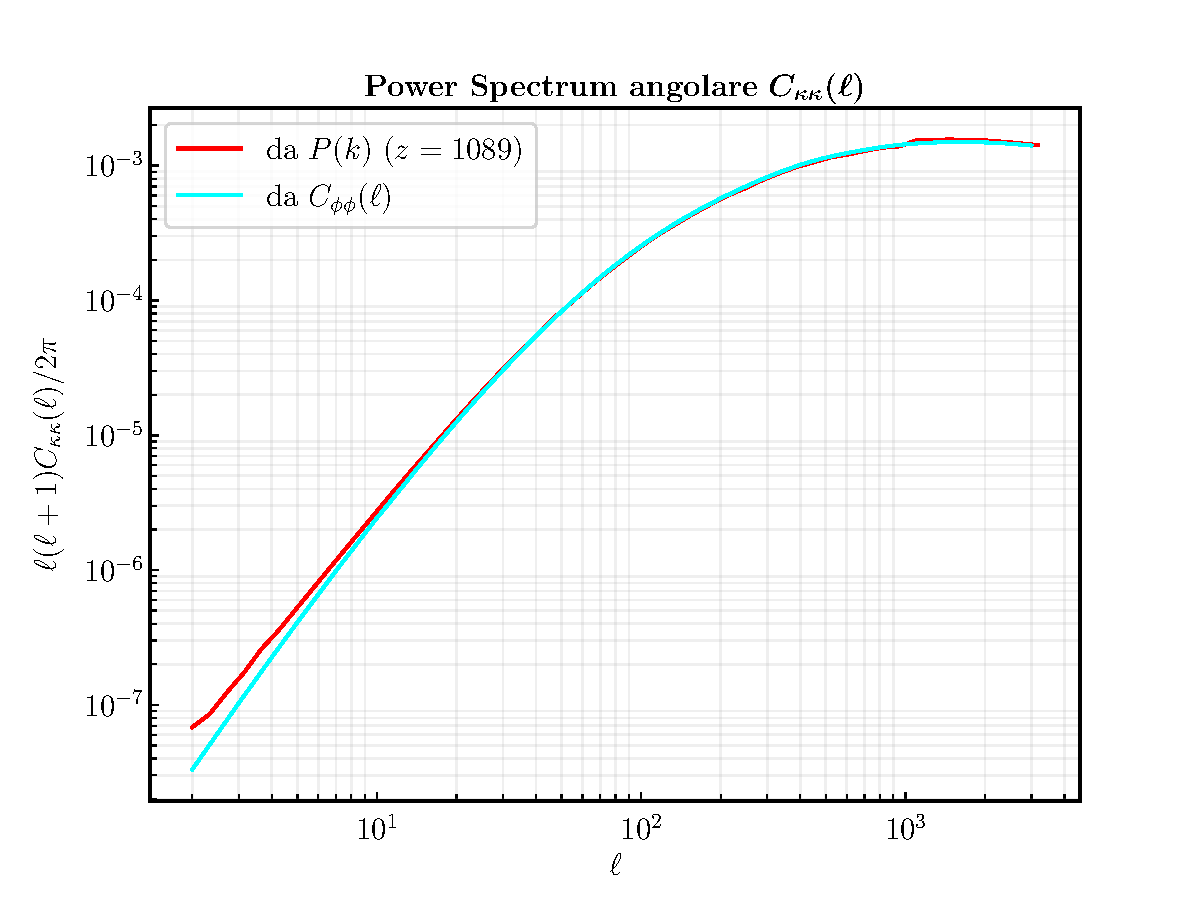
\includegraphics[width=0.6\textwidth]{C_KK_calcolato}
    \caption{Confronto tra $C_{\kappa\kappa}$ calcolato evolvendo lo spettro di potenza della materia e il $C_{\kappa\kappa}$ calcolato dai dati tramite l'equazione \eqref{eq:CKK}.}
\end{figure}

\begin{figure}[ht]
    \centering
    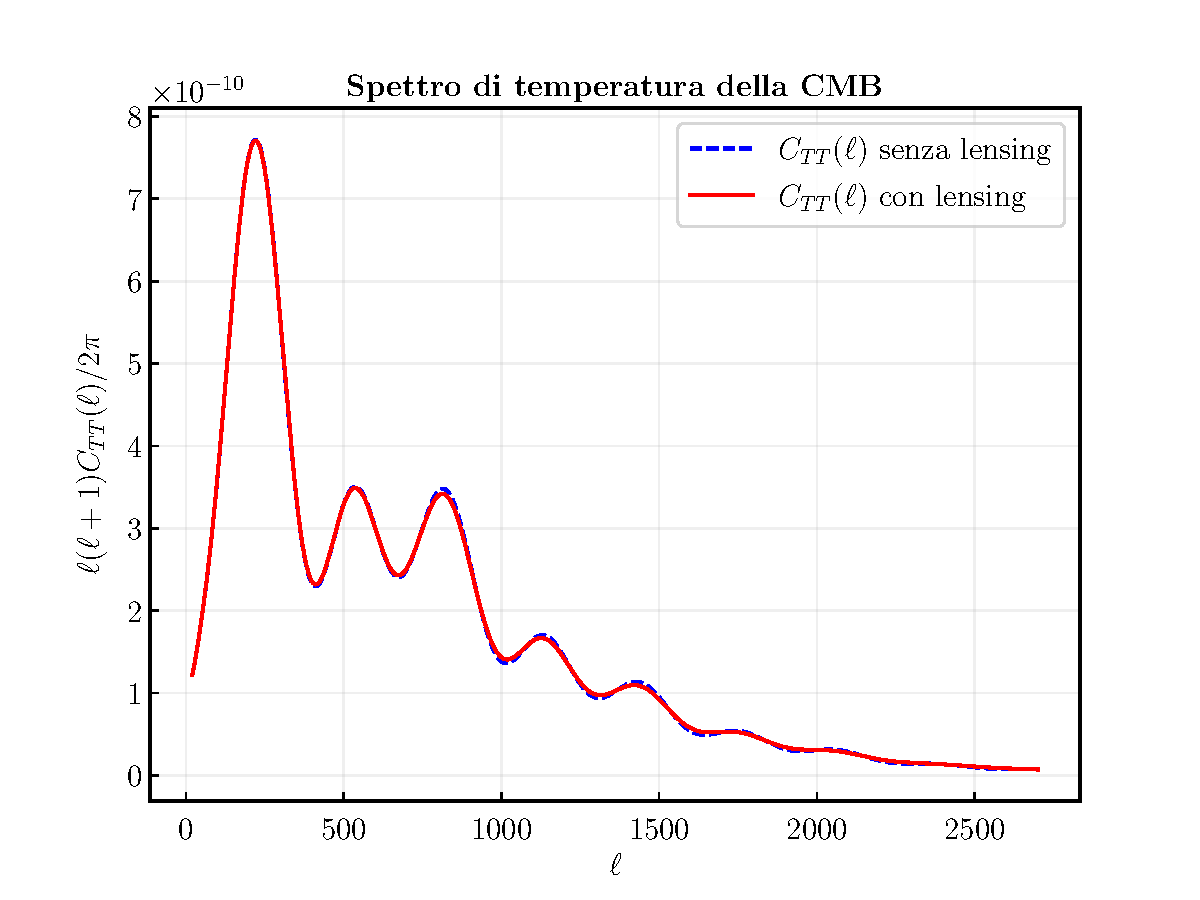
\includegraphics[width=0.6\textwidth]{C_TT}
    \caption{Confronto tra $C_{TT}$ con e senza le correzioni di lensing. Notiamo che il lensing attenua i picchi di potenza.}
\end{figure}

\begin{figure}[ht]
    \centering
    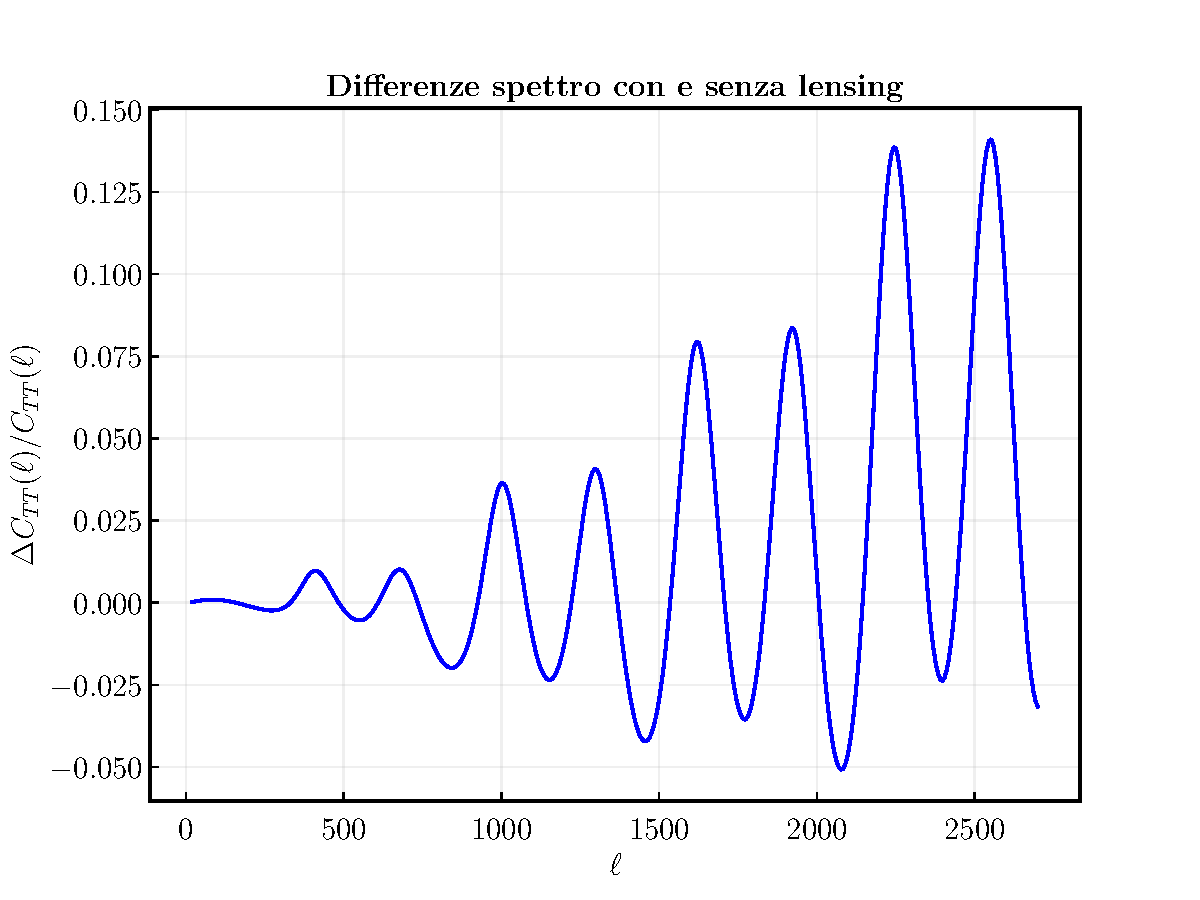
\includegraphics[width=0.6\textwidth]{differenze}
    \caption{Differenza frazionaria tra lo spettro $C_{TT}$ con e senza le correzioni di lensing. Notiamo che il lensing aggiunge potenza sulle piccole scale.}
\end{figure}




\newpage
\subsection{Spettro di potenza della polarizzazione della CMB}

In questo esercizio le correzioni di lensing gravitazionale sono da applicare ai modi di polarizzazione della CMB: il procedimento è qualitativamente lo stesso del punto precedente, dobbiamo però ricavare delle equazioni analoghe alle \eqref{eq:13.21} per il tensore di polarizzazione $I_{ij}$.
Dal'equazione 10.4 del Dodelson, ricordiamo che la componente traceless del tensore di polarizzazione, la quale contiene le informazioni relative agli stati di polarizzazione, è:

\begin{equation} \label{eq:Iij}
    I_{ij}^T = \begin{pmatrix}
                 Q & U \\
                U & - Q
            \end{pmatrix} \ .
\end{equation} 

Scriviamo uno sviluppo in spazio di Fourier analogo all'equazione \eqref{eq:sviluppotheta} per $I_{ij}^T$:

\begin{equation} \label{eq:sviluppoI}
\begin{aligned}
    \tilde I_{ij}^T(\boldsymbol{l}) = & \ I_{ij}^T(\boldsymbol{l}) - \int \frac{d^2 \B l_1}{(2\pi)^2} \boldsymbol{l}_1 \cdot (\B l - \B l_1) \phi_L(\boldsymbol{l}_1) I_{ij}^T(\B l - \B l_1) + \\
        & + \frac{1}{2} \int \frac{d^2 \B l_1}{(2\pi)^2} \int \frac{d^2 \B l_2}{(2\pi)^2} [\B l_1 \cdot (\B l - \B l_1 - \B l_2)] [\B l_2 \cdot (\B l - \B l_1 - \B l_2)] \phi_L(\B l_1) \phi_L(\B l_2) I_{ij}^T(\B l - \B l_1 - \B l_2) \ ,
\end{aligned}
\end{equation}

notando che d'ora in avanti indicheremo con $\tilde A$ una qualsiasi quantità $A$ a cui sono applicate le correzioni di lensing.
A questo punto, ricordiamo che $Q = I_{11}^T = -I_{22}^T$ e $U = I_{12}^T = I_{21}^T$. Inoltre, avendo definito $\B l = l(\cos \varphi_l, \sin \varphi_l)$, dalle equazioni 10.7 e 10.9 del Dodelson possiamo ottenere i modi di polarizzazione $E$ e $B$ come:

\begin{equation} \label{eq:EB}
\begin{cases}
    E(\B l) = Q(\B l) \cos(2\varphi_l) + U(\B l) \sin(2\varphi_l) \\
    B(\B l) = -Q(\B l) \sin(2\varphi_l) + U(\B l) \cos(2\varphi_l) \ .
\end{cases}
\end{equation}

La componente traceless del tensore di polarizzazione diventa dunque:

\begin{equation}
    I_{ij}^{\text{T}}(\boldsymbol{l}) = 
        \begin{pmatrix}
            \cos 2\varphi_l & \sin 2\varphi_l \\
            \sin 2\varphi_l & -\cos 2\varphi_l
            \end{pmatrix} E(\boldsymbol{l}) + 
            \begin{pmatrix}
            -\sin 2\varphi_l & \cos 2\varphi_l \\
            \cos 2\varphi_l & \sin 2\varphi_l
        \end{pmatrix} B(\boldsymbol{l}) \ ,
\end{equation}

e da essa, ricordando la \eqref{eq:Iij}, possiamo ricavare i parametri $Q$ e $U$ in assenza di modi $B$ iniziali:

\begin{equation} \label{eq:QU}
\begin{cases}
    Q(\B l) = E(\B l) \cos(2\varphi') \\
    U(\B l) = E(\B l) \sin(2\varphi') \ .
\end{cases}
\end{equation}

Ora non resta che calcolare i correlatori dei modi $E$ e $B$ ed esprimerli in termini delle componenti di $I_{ij}^T$ per poi utilizzare lo sviluppo \eqref{eq:sviluppoI}.

Calcoliamo lo spettro di potenza con le correzioni di lensing dei modi $E$:

\begin{equation}
    \tilde C_{EE} = \langle \tilde E(\B l) \tilde E(\B l) \rangle = \langle \tilde Q(\B l) \tilde Q(\B l) \rangle \cos^2(2\varphi_l) + 2\langle \tilde Q(\B l) \tilde U(\B l) \rangle \sin(2\varphi_l) \cos(2\varphi_l) + \langle \tilde U(\B l) \tilde U(\B l) \rangle \sin^2(2\varphi_l) \ ,
\end{equation}

dove ricordiamo ancora che $Q = I_{11}^T = -I_{22}^T$ e $U = I_{12}^T = I_{21}^T$ e perciò bisognerà utilizzare le componenti corrispondenti dello sviluppo \eqref{eq:sviluppoI}.
Per i correlatori presenti in questa equazione, valgono le equazioni \eqref{eq:13.21} sostituendo $C(l)$ con il corrispondente spettro imperturbato, calcolato con $B=0$ mediante la \eqref{eq:QU}:

\begin{itemize}
    
    \item $C_{QQ}(l) = \langle E(\B l) E(\B l) \rangle \cos^2(2\varphi') = C_{EE}(l) \cos^2(2\varphi')$

    \item $C_{QU}(l) = \langle E(\B l) E(\B l) \rangle \sin(2\varphi') \cos(2\varphi') = C_{EE}(l) \sin(2\varphi') \cos(2\varphi')$
    
    \item $C_{UU}(l) = \langle E(\B l) E(\B l) \rangle \sin^2(2\varphi') = C_{EE}(l) \sin^2(2\varphi')$ \ .

\end{itemize}

Poiché tutti i correlatori imperturbati dipendono da $C_{EE}$, definiamo i coefficienti della prima equazione delle \eqref{eq:13.21} per la polarizzazione come:

\begin{itemize}
    
    \item $\displaystyle C_{EE}^{(22)}(l) = \int \frac{d^2 \B l_1}{(2\pi)^2} \left[ \boldsymbol{l}_1 \cdot (\boldsymbol{l} - \boldsymbol{l}_1) \right]^2 C_{\phi\phi}(l_1) C_{EE}(|\boldsymbol{l} - \boldsymbol{l}_1|)$
    
    \item $\displaystyle C_{EE}^{(13)}(l) = -\frac{1}{4} \left[ \int \frac{d^2 \B l_1}{(2\pi)^2} l_1^2 C_{\phi\phi}(l_1) \right] l^2 C_{EE}(l)$ .

\end{itemize}

Perciò, omettendo le dipendenze da $l$, abbiamo:

\begin{equation}
\begin{aligned}
    &\tilde C_{EE} = [ C_{EE} \cos^2(2\varphi_l) + C_{EE}^{(22)} \cos^2(2\varphi_{l-l_1}) + 2C_{EE}^{(13)} \cos^2(2\varphi_l) ] \cos^2(2\varphi_l) + \\
        & + 2 [ C_{EE} \sin(2\varphi_l)\cos(2\varphi_l) + C_{EE}^{(22)} \sin(2\varphi_{l-l_1})\cos(2\varphi_{l-l_1}) + 2C_{EE}^{(13)} \sin(2\varphi_l)\cos(2\varphi_l) ] \sin(2\varphi_l)\cos(2\varphi_l) + \\
        & + [ C_{EE} \sin^2(2\varphi_l) + C_{EE}^{(22)} \sin^2(2\varphi_{l-l_1}) + 2C_{EE}^{(13)} \sin^2(2\varphi_l) ] \sin^2(2\varphi_l) \ ,
\end{aligned}
\end{equation}

dove i termini trigonometrici dipendenti da $\B l_1$ sono da intendersi dentro agli integrali contenuti nelle definizioni di $C_{EE}^{(22)}$ e $2C_{EE}^{(13)}$.
Raccogliendo dunque i termini $C_{EE}$, $C_{EE}^{(22)}$ e $2C_{EE}^{(13)}$, lo spettro diventa:

\begin{equation}
\begin{aligned}
    &\tilde C_{EE} = C_{EE} [ \cos^4(2\varphi_l) + 2\sin^2(2\varphi_l)\cos^2(2\varphi_l) + \sin^4(2\varphi_l) ] + \\
        & + C_{EE}^{(22)} [ \cos^2(2\varphi_{l-l_1}) \cos^2(2\varphi_l) + 2\sin(2\varphi_{l-l_1})\cos(2\varphi_{l-l_1}) \sin(2\varphi_l)\cos(2\varphi_l) + \sin^2(2\varphi_{l-l_1}) \sin^2(2\varphi_l) ] + \\
        & + 2C_{EE}^{(13)} [ \cos^4(2\varphi_l) + 2\sin^2(2\varphi_l)\cos^2(2\varphi_l) + \sin^4(2\varphi_l) ] \ .
\end{aligned}
\end{equation}

Le parentesi del primo e del terzo termine restituiscono $[\sin^2(2\varphi_l) + \cos^2(2\varphi_l)]^2 = 1$, mentre quella del secondo termine diventa:

\begin{equation}
    [\cos(2\varphi_{l-l_1})\cos(2\varphi_l) + \sin(2\varphi_{l-l_1})\sin(2\varphi_l)]^2 = \cos^2[2(\varphi_{l-l_1} - \varphi_l)] \ .
\end{equation}

Perciò lo spettro dei modi $E$ con le correzioni di lensing è:

\begin{equation} \label{eq:EE}
\begin{aligned}
    \tilde C_{EE}(l) =& \ C_{EE}(l) + \int \frac{d^2 \B l_1}{(2\pi)^2} \left[ \boldsymbol{l}_1 \cdot (\boldsymbol{l} - \boldsymbol{l}_1) \right]^2 C_{\phi\phi}(l_1) C_{EE}(|\boldsymbol{l} - \boldsymbol{l}_1|) \cos^2[2(\varphi_{l-l_1} - \varphi_l)] + \\
        & -\frac{1}{2} \left[ \int \frac{d^2 \B l_1}{(2\pi)^2} l_1^2 C_{\phi\phi}(l_1) \right] l^2 C_{EE}(l) \ .
\end{aligned}
\end{equation}

Veniamo ora al calcolo dello spettro di potenza con le correzioni di lensing relativo ai modi $B$ di polarizzazione della CMB.
Il calcolo è del tutto analogo a quello svolto per i modi $E$:

\begin{equation}
\begin{aligned}
    &\tilde C_{BB} = \langle \tilde B(\B l) \tilde B(\B l) \rangle = \langle \tilde Q(\B l) \tilde Q(\B l) \rangle \sin^2(2\varphi_l) - 2\langle \tilde Q(\B l) \tilde U(\B l) \rangle \sin(2\varphi_l) \cos(2\varphi_l) + \langle \tilde U(\B l) \tilde U(\B l) \rangle \cos^2(2\varphi_l) = \\
        & = C_{EE} [ \sin^2(2\varphi_l)\cos^2(2\varphi_l) - 2\sin^2(2\varphi_l)\cos^2(2\varphi_l) + \sin^2(2\varphi_l)\cos^2(2\varphi_l) ] + \\
        & + C_{EE}^{(22)} [ \sin^2(2\varphi_l)\cos^2(2\varphi_{l-l_1}) - 2\sin(2\varphi_{l-l_1})\cos(2\varphi_{l-l_1}) \sin(2\varphi_l)\cos(2\varphi_l) + \sin^2(2\varphi_{l-l_1})\cos^2(2\varphi_l) ] + \\
        & + C_{EE}^{(13)} [ \sin^2(2\varphi_l)\cos^2(2\varphi_l) - 2\sin^2(2\varphi_l)\cos^2(2\varphi_l) + \sin^2(2\varphi_l)\cos^2(2\varphi_l) ] \ .
\end{aligned}
\end{equation}

La prima e la terza parentesi si annullano, mentre la seconda diventa:

\begin{equation}
    [\cos(2\varphi_{l-l_1})\sin(2\varphi_l) - \sin(2\varphi_{l-l_1})\cos(2\varphi_l)]^2 = \sin^2[2(\varphi_{l-l_1} - \varphi_l)] \ .    
\end{equation}

Dunque lo spettro dei modi $B$ di polarizzazione della CMB con le correzioni di lensing diventa:

\begin{equation} \label{eq:BB}
    \tilde C_{BB}(l) = \int \frac{d^2 \B l_1}{(2\pi)^2} \left[ \boldsymbol{l}_1 \cdot (\boldsymbol{l} - \boldsymbol{l}_1) \right]^2 C_{\phi\phi}(l_1) C_{EE}(|\boldsymbol{l} - \boldsymbol{l}_1|) \sin^2[2(\varphi_{l-l_1} - \varphi_l)] \ .
\end{equation}

Facciamo ora una precisazione sugli angoli utilizzati nelle precedenti equazioni.
Data la definizione di $\B l$:

\begin{equation}
    \B l = l(\cos \varphi_l, \sin \varphi_l) \ ,
\end{equation}

l'angolo $\varphi_l$ è dato da $\varphi_l = \arctan(l_y/l_x)$ e in un sistema di assi cartesiani esso è l'angolo tra il vettore $\B l$ e l'asse $x$.
Dato ora un secondo vettore $\B l_1$, chiamiamo $\theta$ l'angolo tra $\B l_1$ ed $\B l$, e $\varphi_{l_1}$ l'angolo tra $\B l_1$ e l'asse $x$.
Infine, la differenza vettoriale $\B l - \B l_1$, definisce un altro angolo, $\varphi_{l-l_1}$, ossia l'angolo tra il vettore differenza $\B l - \B l_1$ e l'asse $x$, dato da:

\begin{equation}
    \varphi_{l-l_1} = \arctan \left[ \frac{ l \sin \varphi_{l_1} \cos \theta - l \cos \varphi_{l_1} \sin \theta - l_1 \sin \varphi_{l_1} }{ l \cos \varphi_{l_1} \cos \theta + l \sin \varphi_{l_1} \sin \theta - l_1 \cos \varphi_{l_1} } \right] \ .
\end{equation}

Scegliendo arbitrariamente $\B l$ lungo l'asse $x$, ottengo che $\varphi_l = 0$, $\varphi_{l_1} = \theta$ e:

\begin{equation}
    \varphi_{l-l_1} = \arctan \left[ \frac{l_1 \sin \varphi_{l_1}}{l_1 \cos \varphi_{l_1} -l} \right] \ .
\end{equation}

Computazionalmente il problema è del tutto analogo al punto precedente: l'obiettivo è quello di calcolare gli spettri con le correzioni di lensing dei modi $E$ \eqref{eq:EE} e $B$ \eqref{eq:BB} della polarizzazione della CMB.

Abbiamo affrontato l'esercizio nello stesso Jupyter Notebook del punto precedente, lasciamo nuovamente il link per la repository di GitHub contenente tutto il materiale: \href{https://github.com/ste-cartu/Fisica-Gravitazionale-Avanzata}{\faIcon{github}}.

Di seguito riportiamo alcuni plot ottenuti.

\newpage
\begin{figure}[ht]
    \centering
    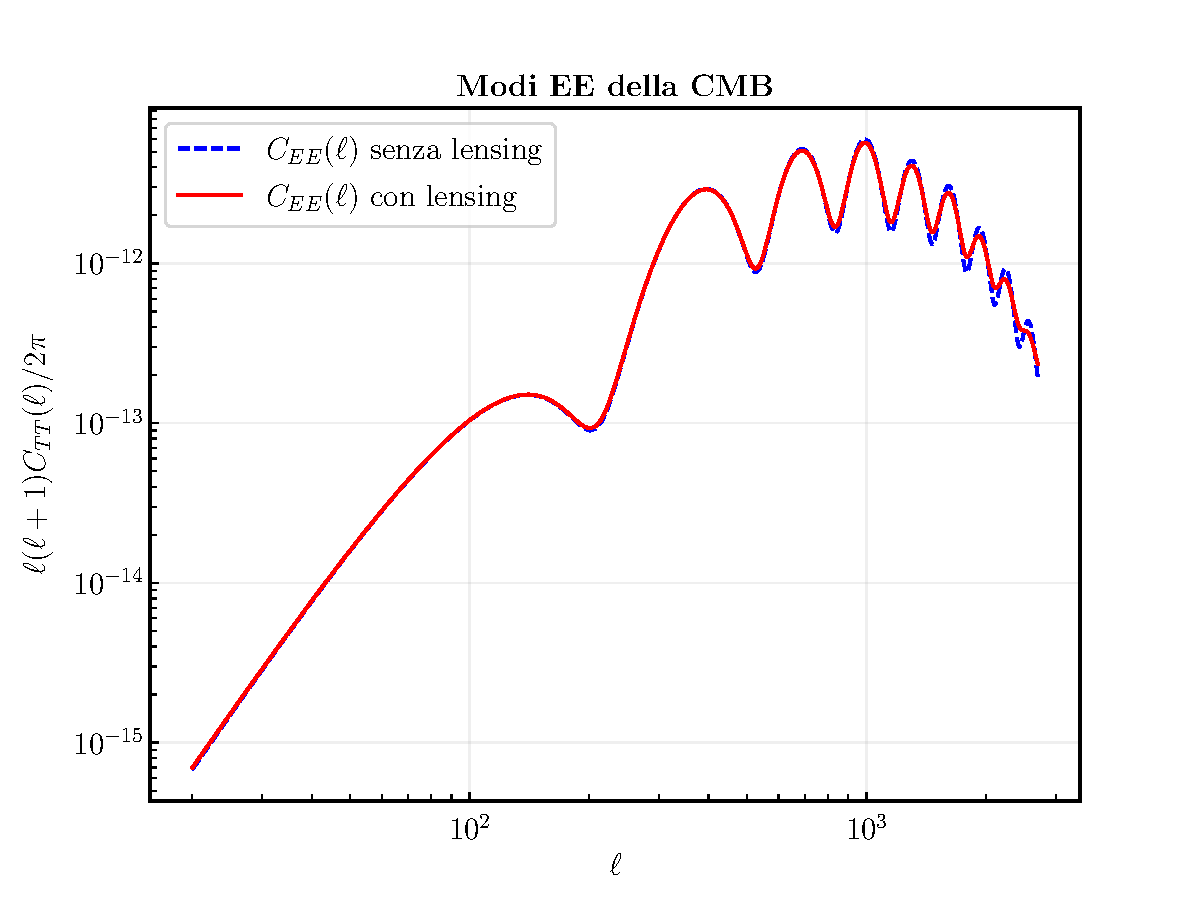
\includegraphics[width=0.6\textwidth]{C_EE}
    \caption{Confronto tra $C_{EE}$ con e senza le correzioni di lensing.}
\end{figure}

\begin{figure}[ht]
    \centering
    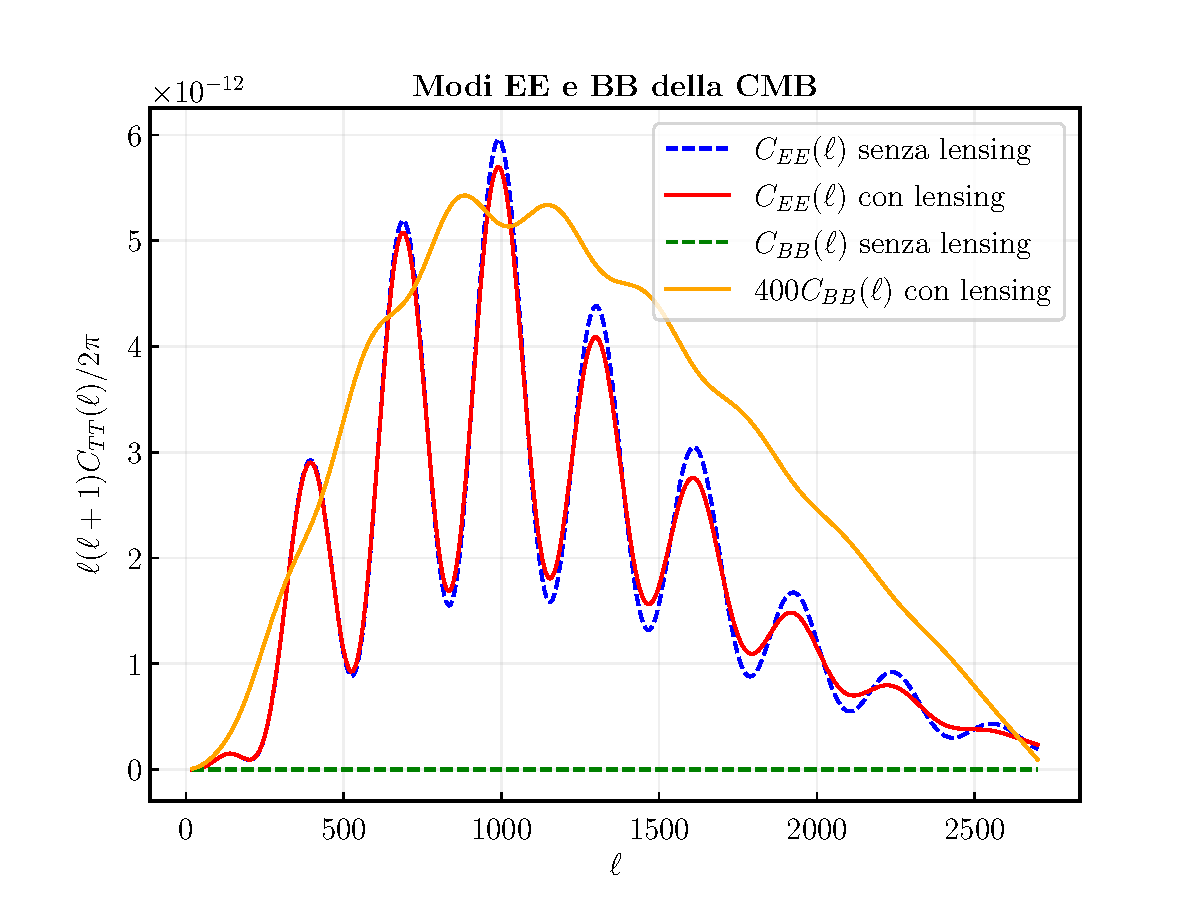
\includegraphics[width=0.6\textwidth]{modi}
    \caption{Confronto tra i vari modi di polarizzazione della CMB, con e senza le correzioni di lensing.}
\end{figure}


\end{document}